% Candidate source: src-0f11f5c9f471004d5361ba63a8cd76e404c5e126be072fcfb0e205938017cbb2
% Source PDF SHA-256: 2e925ec0caa385c49600a41d3e05877c7c9e7fe13d37904274de8c389e4fd79b
% PDF page 1 (printed page 208), question 10.
% Redraw follows visible/hidden edges: regular triangular prism ABC-A1B1C1, point D on BB1, lines AD and C1A.
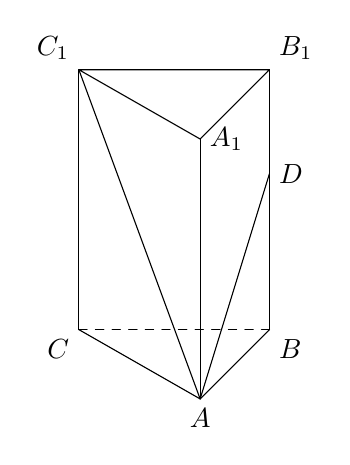
\begin{tikzpicture}[line cap=round,line join=round,>=latex,scale=1.1]
  % Bottom face vertices
  \coordinate (C) at (0,0);
  \coordinate (B) at (2.2,0);
  \coordinate (A) at (1.4,-0.8);

  % Top face vertices (vertical shift 3.0)
  \coordinate (C1) at (0,3.0);
  \coordinate (B1) at (2.2,3.0);
  \coordinate (A1) at (1.4,2.2);

  % Point D on BB1
  \coordinate (D) at (2.2,1.8);

  % Hidden edges
  \draw[dashed] (C) -- (B);

  % Visible edges: bottom face
  \draw (C) -- (A) -- (B);

  % Visible edges: top face
  \draw (C1) -- (A1) -- (B1) -- cycle;

  % Lateral edges
  \draw (C) -- (C1);
  \draw (B) -- (B1);
  \draw (A) -- (A1);

  % Connecting lines AD and C1A
  \draw (A) -- (D);
  \draw (C1) -- (A);

  % Vertex labels
  \node[below left] at (C) {$C$};
  \node[below right] at (B) {$B$};
  \node[below] at (A) {$A$};
  \node[above left] at (C1) {$C_1$};
  \node[above right] at (B1) {$B_1$};
  \node[right] at (A1) {$A_1$};
  \node[right] at (D) {$D$};
\end{tikzpicture}
